
\section{Linear Classification}
For classification problem, in this section we assume the classification boundaries are linear, i.e., in the input hyperspace the points belonging to different classes can be separated by hyperplanes. 

\subsection{Linear regression of an Indicator matrix}
Suppose we have $K$ classes. For a single output we build a vector $\mathbf{y} = \left( y_1, \cdots, y_k\right)$ where $y_k=1$ if the class it belongs is the $k$ class. As output we will have the matrix $\mathbf{Y}$ of $0$ and $1$ with each row having a single $1$. We fit a linear regression model to each of the columns of $\mathbf{Y}$ simultaneously:
\begin{align*}
\hat{\mathbf{Y}} = \mathbf{X}\left( \mathbf{X}^T\mathbf{X}\right)^{-1}\mathbf{X}^T\mathbf{Y}
\end{align*}
We get a coefficient vector for each response column $y_k$, and hence a $(p+1) \times K$ matrix $\hat{\mathbf{B}} = \left( \mathbf{X}^T\mathbf{X}\right)^{-1}\mathbf{X}^T\mathbf{Y}$,where $\mathbf{X}$ will have $p+1$ columns with a leading column of 1 for the intercept.

Suppose we are given a new input $x$. Then the classification problem becomes:

\textit{compute the output $\hat{f}(x)^T = (1, x^T)\mathbf{\hat{B}}$ which is a $k$ vector
identify the largest component $\hat{G}(x) = \argmax{k \in \mathcal{G}} \hat{f}_k(x)$}.

With this approach we are basically estimating a conditional expectation, i.e., given the inputs $\x$ what is the probability the output is of class $k$? Mathematically $\E\left( y_k|X=x\right) =  Pr\left( G=k|X=x\right)$ since $y_k=1$.

Although the linear model guarantees $\sum_{k \in \mathcal{G}}\hat{f}_k=1$, as long as there is an intercept in the model, $\hat{f}_k(x)$ can be negative or bigger than one, especially when making predictions outside the hull of training data. Although this fact, this approach still works in many cases.

\textbf{An important limitation} is when $K\ge 3$. Even if the classes can still be separated by more than one linear boundaries, linear regression cannot find linear boundaries (because they are more than one?).

Quadratic regression might solve the problem, but a general rule is that if $k\ge3$ classes are lined up (their centroids are in the same line), a polynomial term with degree up to $k-1$ is  needed to solve the problem, and since the direction is arbitrary, cross-products terms might be needed too.

\subsection{Linear Discriminant analysis}
\label{LDA}
For optimal classification we have to know the class posteriors $Pr\left( G|X\right)$. Let $\pi_k$ be the prior probability of class $k$ with $\sum_k^K \pi_k=1$. Suppose $f_k(x)$ is the class conditional density.
From the Bayes theorem (?) we get 
\begin{equation}
Pr\left( G=k | X=x\right) = \frac{Pr\left( X=x |G=k \right)Pr(G=k)}{Pr(X=x)}
\end{equation}
% 
$Pr(G=k)$ is the prior probability $\pi_k$, $Pr\left( X=x |G=k \right)$ is the class conditional density while the denominator can be rewritten using the \textbf{Total Probability Theorem} as
\begin{align}
&Pr(X=x) = \sum_{l=1}^{K} Pr(X=x|G=l) Pr(G=l) = \sum_{l=1}^{K} Pr(X=x|G=l) \pi_\ell\\
&\Rightarrow Pr\left( G=k | X=x\right) =\frac{f_k(x)\pi_k}{\sum_{l=1}^Kf_\ell(x)\pi_\ell}
\end{align}

The goodness of classification mostly rely on $f_k(x)$ and many techniques use models for class densities:
\begin{itemize}
\item linear and quadratic discriminant analysis use Gaussian densities;
\item mixtures of Gaussians allow for non-linear boundaries;
\item Naive Bayes models assume that each class density is a product of marginal densities i.e., inputs are conditionally independent in each class.
\end{itemize}
Modelling each class density as a multivariate Gaussian we have
\begin{equation}
f_k(x) = \frac{1}{(2\pi)^{\frac{p}{2}}|\sum_k|^{\frac{1}{2	}}} e^{-\frac{1}{2}\left( x-\mu_k\right)^T\Sigma_k^{-1}\left( x-\mu_k\right)}
\end{equation}

\textbf{Linear Discriminant analysis assumes equal covariance matrices for all classes}. Taking as comparison between two classes the log-ratio, we have
\begin{equation}
\begin{aligned}
\log &\frac{Pr(G=k|X=x)}{Pr(G=l|X=x)} = \log \frac{f_k(x) \pi_k}{f_\ell(x) \pi_\ell} = \log \frac{ \pi_k}{ \pi_\ell} + \log\frac{f_k(x)}{f_\ell(x) } =\\
&= \log \frac{ \pi_k}{ \pi_\ell} + \log\frac{e^{-\frac{1}{2}\left( x-\mu_k\right)^T\Sigma^{-1}\left( x-\mu_k\right)}}{e^{-\frac{1}{2}\left( x-\mu_\ell\right)^T\Sigma^{-1}\left( x-\mu_\ell\right)} }   =  \\
&=log \frac{ \pi_k}{ \pi_\ell} - \frac{1}{2}\left( x-\mu_k\right)^T\Sigma^{-1}\left( x-\mu_k\right) - \left( -\frac{1}{2}\right)\left( x-\mu_\ell\right)^T\Sigma^{-1}\left( x-\mu_\ell\right) =\\
&= log \frac{ \pi_k}{ \pi_\ell} - \frac{1}{2}\left[\left( x-\mu_k\right)^T\Sigma^{-1}\left( x-\mu_k\right) + \left( x-\mu_\ell\right)^T\Sigma^{-1}\left( \mu_\ell - x\right)\right] =\\
&= log \frac{ \pi_k}{ \pi_\ell} - \frac{1}{2}\left[\left( 2x-\mu_k-\mu_\ell\right)^T\Sigma^{-1}\left( \mu_\ell-\mu_k\right) \right] =\\
&= log \frac{ \pi_k}{ \pi_\ell} +\frac{1}{2}x^T\Sigma^{-1}\left( \mu_k-\mu_\ell\right)- \frac{1}{2}\left( \mu_k+\mu_\ell\right)^T\Sigma^{-1}\left( \mu_k-\mu_\ell\right) =\\
\end{aligned}
\end{equation}
which is linear in $x$, so all decision boundaries are linear (i.e., they are hyperplanes in $p$ dimensions). If the common covariance matrix is spherical, i.e., $\Sigma=\sigma^2 I$ and the class priors are equal, each boundary that separates two classes is the perpendicular bisector of the segment joining the centroids of the two classes.

The linear discriminant functions of each class are 
\begin{equation}
\delta_k(x)  = x^T \Sigma^{-1}\mu_k -\frac{1}{2}\mu_k^T+log\pi_k
\end{equation}
We do not know the parameters of the Gaussian distribution and we must estimate them from the training data:
\begin{align}
&\hat{\pi}_k = \frac{N_k}{N}\\
&\hat{\mu}_k = \sum_{g_i=k}\frac{x_i}{N_k}\\
&\hat{\Sigma} = \sum_{k=1}^K\frac{(x_i-\hat{\mu}_k)(x_i-\hat{\mu}_k)^T}{(N-K)}
\end{align}

\textbf{Note} that LDA does not use Gaussian assumption for the features.

\subsubsection{Decision rule}
Consider two classes $1$ and $2$. LDA classifies to class $1$ if
\begin{equation}
x^T\hsi \hmu_1 - \frac{1}{2}\hmu_1^T\hsi\hmu_1 + \log \hpi_1 >x^T\hsi \hmu_2 - \frac{1}{2}\hmu_2^T\hsi\hmu_2 + \log \hpi_2
\end{equation}
to class $2$ if $<$ holds. In such case there is a correspondence between LDA and linear regression classification if the two classes are coded with $+1$ and $-1$. In this case the coefficient vector from least squares is proportional to the LDA direction. However unless $N_1=N_2$, the intercepts are different and so are the decision rules.

With more than $2$ classes, linear regression is not able to classify correctly while LDA does.

\subsection{Quadratic Discriminant analysis}
If we do not assume equal covariance, the squared term in $x$ does not cancel out and we get quadratic discriminant functions:
\begin{equation}
\label{QDA}
\begin{aligned}
\delta_k  (x) &= -\frac{1}{2} \log |\Sigma_k| -\frac{1}{2} \left( x - \mu_k \right)^T \si_k\left( x - \mu_k \right) + \log \pi_k
\end{aligned}
\end{equation}
The decision boundaries between two classes are quadratic functions.

\textbf{Note}: QDA does not differ much from LDA applied the enlarged quadratic polynomial input space but generally QDA is preferred in this case.

The estimates are similar but the covariance matrix must be estimated for each class. When $p$ is large, this means a dramatic increase in the number of parameters, considering we only need the differences $\delta_k (x) - \delta_\ell(x)$. LDA needs $(K-1)\times (p+1)$ parameters, while QDA needs $(K-1) \times \left(p\left(p+3\right)/2 +1\right)$.

\subsection{Regularized discriminant analysis}
This method shrinks the separate covariances of QDA towards a common covariance as in LDA. In a way it is similar to ridge regression. The regularized covariance matrices have the form:

\begin{equation}
\hS_k(\alpha) = \alpha\hS_k+(1-\alpha) \hS
\end{equation}
with $\alpha \in [0,1]$, the two extremes being LDA and QDA. $\alpha$ can be chosen on the validation data or by cross-validation.

Similarly we can allow $\hS$ to be shrunk toward the scalar covariance:
\begin{equation}
\hS(\gamma) = \gamma\hS+(1-\gamma) \hat{\sigma}^2 I
\end{equation}
with $\gamma \in [0,1]$
so we get a more general family of covariances
\begin{equation}
\hS_k(\alpha, \gamma) = \alpha\hS_k+\left(1-\alpha\right) \left(\gamma\hS+\left(1-\gamma\right) \hat{\sigma}^2 I\right)
\end{equation}

\subsection{Computation}
Computation of LDA and QDA is simplified by diagonalizing the covariance matrices with the singular value decomposition $\hS_k = U_kD_kU_k^T$. The terms in \autoref{QDA} become
\begin{align}
&\begin{aligned}
&\left( x - \mu_k \right)^T \si_k\left( x - \mu_k \right)= \left( x - \mu_k \right)^T \left(U_kD_kU_k^T\right)^{-1}\left( x - \mu_k \right) =\\
&= \left( x - \mu_k \right)^T U_kD_k^{-1}U_k^T\left( x - \mu_k \right) =  \left[ U_k^T\left( x - \mu_k \right)\right]^T D_k^{-1}\left[ U_k^T\left( x - \mu_k \right)\right]
\end{aligned}\\
& \log |\hS_k| = \sum_\ell \log d_{kl}
\end{align}
Considering the above steps, LDA classifier can be seen as performing the following steps:
\begin{itemize}
\item sphere the data w.r.t. the common covariance estimate: $X*\leftarrow D^{-\frac{1}{2}} U^T X$. The common covariance estimate of $X*$ will now be the identity.
\item Classify to the closest centroid in the transformed space, modulo the effect of the class prior probability $\pi_k$(?)
\end{itemize}
\subsection{Regularized-rank linear discriminant analysis}
Consider $K=2$ with two centroids and the input is $2$, i.e., input points are on a plane. Given an input point, for classification purposes what matters is not the distance in the $p$ space of such point from the two centroids but rather the distance from the two centroids of the projection of this point on the line joining them (\autoref{proj}). So basically instead of using the $2$ dimensions, we are calculating the distance in one dimension, a line. If $K=3$ then the points are projected onto a plane (2d), of course in this case it is convenient if $p>2$.

More generally the $K$ centroids in $p$-dimensional input, lie in an affine subspace of dimensions $\le K-1$ and if $p>$ is much larger than $K$ this will be a considerable drop in dimension.


\begin{figure}
\centering
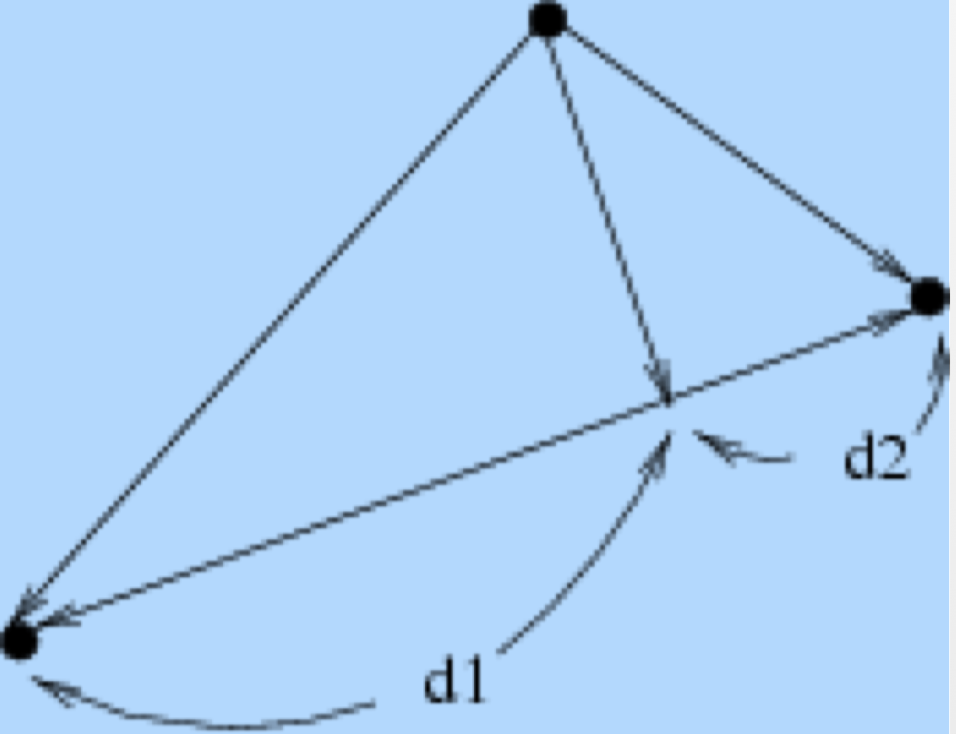
\includegraphics[scale=0.4]{img/proj}
\caption{...}
\label{proj}
\end{figure}

If $K>3$ we can look for a $L<K-1$ dimensional subspace optimal for LDA. Fisher defined \textit{optimal} such that the projected centroids were spread out as much as possible in terms of variance.
This problem, finding the principal component subspaces of the centroids, involves the following steps:
\begin{itemize}
\item compute the $k\times p$ matrix of class centroids $M$ and the common covariance matrix $W$ for within-class covariance;
\item compute $M*=MW^{-\frac{1}{2}}$ using the eigen-value decomposition;
\item compute $B*$, the covariance matrix of $M*$ ($B$ for between class covariance) and its eigenvalue decomposition $B^{*}=V^{*}D_BV^{*T}$. The columns $v^*_\ell$ from the first to the last define the coordinates of optimal subspaces.
\end{itemize}
The $lth$ discriminant variable is given by $Z_\ell =  v_\ell^TX$ with $v_\ell=W^{-\frac{1}{2}} v^*_\ell$.  Although the direction joining the centroids separates the means as much as possible(maximizes the between class covariance), there is an overlap between the projected classes due to the nature of covariances. Taking the covariances into account reduce the overlap and that is what we are doing (\autoref{cov}).

\begin{figure}
\centering
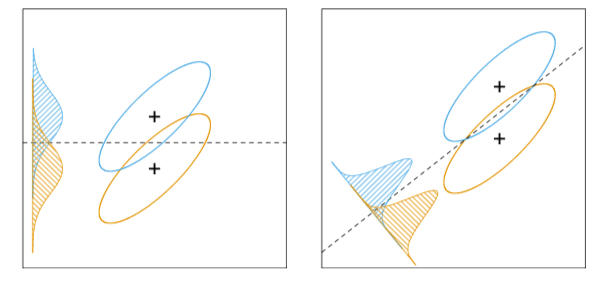
\includegraphics[scale=0.4]{img/cov}
\caption{Covariance.}
\label{cov}
\end{figure}

The between-class variance $Z$ is $a^TBa$ and the within class variance is $a^TWa$, with $B+W=T$, the total covariance matrix of $X$.
Fisher's problem maximizes the \textit{Rayleigh quotient}:

\begin{equation}
max_{a} \frac{a^TBa}{a^TWa}
\end{equation}

This is a generalized eigenvalue problem, with $a$ given by the largest eigenvalue. Similarly one can find the next direction $a_2$, orthogonal in $W$ to $a_1$, such that $a^T_2 Ba_2/a^T_2 Wa_2$ is maximized; the solution is a$_2 = v_2$, and so on. $a_\ell$ are the \textit{discriminant coordinates} or \textit{canonical variates}, different from discriminant functions.

The reduced subspaces can be used both for visualization and classification by limiting the distance between centroids to the chosen subspace. However, when doing this, due to the Gaussian classification, a correction factor of $\log \pi_k$ is needed. The misclassification is given by the overlapping area in \autoref{cov} between the two densities. When both classes have the same priors $\pi_k$ as in the figure, the optimal cut-point is the midway between projected means, if not the cut-point is moved towards the smaller class to have a better error rate.

For $2$ classes one can derive the linear rule using LDA, and then choosing the cut-point to minimize misclassification error.

\subsection{Logistic regression}
\label{LogReg}
The idea behind logistic regression is to still exploit a linear model $x^T\beta$ but having its output representing a probability, i.e., constrained between $0$ and $1$. This part is performed using the \tb{sigmoid function}:

\begin{equation}
p=\sigma(q) = \frac{1}{1+e^{-q}}.
\end{equation}
Inverting the terms we get 
\begin{equation}
\label{logit}
q = -\log\frac{1-p}{p} = \log \frac{p}{1-p} 
\end{equation}
\autoref{logit} is called \textbf{logit function}. As $q$ increases to $\infty$, the output of the sigmoid gets closer to $1$; instead when it diverges to $-\infty$ we get $0$. Suppose we have just 2 classes or equivalently a binary classifier that tells the probability of an event to happen: $Y_n=1$ when the event happens and $Y_n=0$ when it does not. We can express the probabilities output by our classifier when new input data $x_{new}$ are observed as:
\begin{equation}
\begin{aligned}
&P(G=1|x_n, \beta) =  \frac{1}{1+e^{-\beta^T\x_{new}}}\\
&P(G=0|x_n, \beta) = 1- \frac{1}{1+e^{-\beta^T\x_{new}}} = \frac{e^{-\beta^T\x_{new}}}{1+e^{-\beta^T\x_{new}}}
\end{aligned}
\end{equation}

These equations can be combined in a single equation:
\begin{equation}
P(G=g|x_n, \beta) =  P(G=1|x_n, \beta)^{g} P(G=0|x_n, \beta)^{g-1}
\end{equation}

Taking the log-ratio between the two probabilities we have:
\begin{equation}
\begin{aligned}
\log \frac{P(Y_n=0|x_n, \beta)}{P(Y_n=1|x_n, \beta)} =  \log \frac{\frac{e^{-\beta^T\x_{new}}}{\cancel{1+e^{-\beta^T\x_{new}}}}}{\frac{1}{\cancel{1+e^{-\beta^T\x_{new}}}}} = -\beta^T\x_{new}
\end{aligned}
\end{equation}
So we are using lines (or hyperplanes) to separate the two classes.

\subsubsection{Multinomial logistic regression: more than 2 classes}
Now suppose we have more than two classes and we still want to separate those classes with linear functions, which means we will have a hyperplane separating two classes. We have $K$ possible outcomes. We can think to run $K-1$ independent binary logistic regressions with one class chosen as \textbf{pivot}, generally the one corresponding to class $K$, and with the other $K-1$ classes separately regressed against the pivot:
%LR models the posterior probabilities of the classes as linear function in $x$, while ensuring they sum up to $1$.
%The model has the form
\begin{equation}
\begin{aligned}
&\log \frac{Pr\left(G=1|X=x\right)}{Pr\left(G=K|X=x\right)} = \beta_1^T x \\
&\log \frac{Pr\left(G=2|X=x\right)}{Pr\left(G=K|X=x\right)} = \beta_2^T x\\
\vdots\\
&\log \frac{Pr\left(G=K-1|X=x\right)}{Pr\left(G=K|X=x\right)} = \beta_{\left(K-1\right)}^T x
\end{aligned}
\label{logratio}
\end{equation}
The choice of the pivot class used as denominator is arbitrarily and the estimates are equivalent under different choices.

Summing the probability of each class we must get $1$:
\begin{equation}
\begin{aligned}
&\sum_{\ell=1}^{K} Pr\left(G=\ell|X=x\right) = 1 \Rightarrow Pr\left(G=K|X=x\right)+ \sum_{\ell=1}^{K-1} Pr\left(G=\ell|X=x\right)=1\\
&\Rightarrow Pr\left(G=K|X=x\right) +\sum_{\ell=1}^{K-1} Pr\left(G=K|X=x\right)e^{\beta_\ell^Tx}=1\\
&\Rightarrow Pr\left(G=K|X=x\right) \br{1+\sum_{\ell=1}^{K-1} e^{\beta_\ell^Tx}}=1\\
&\Rightarrow Pr\left(G=K|X=x\right)= \frac{1}{1+\sum_{\ell=1}^{K-1} e^{\beta_\ell^Tx}}
\end{aligned}
\end{equation}
where the \autoref{logratio} has been substituted in.
So we can re-express the probabilities as:

\begin{equation}
Pr\left(G=k|X=x\right) = \frac{e^{\beta_{k}^T x}}{1+\sum_{\ell=1}^{K-1} e^{\beta_\ell^Tx}}
\end{equation}

Note that the boundaries between any two classes are linear:
\begin{equation*}
\log \frac{Pr(G=i|X=x)}{Pr(G=j|X=x)} = \log \frac{e^{\beta_i^T x}}{e^{\beta_j^T x}} = \br{\beta_i -\beta_j}x
\end{equation*}

\subsubsection{Another approach: the softmax function}
\label{sssec:softmax}
As already stated we want linear boundaries between classes. This means that for any pair of classes:
\begin{equation}
\log \frac{Pr\left(G=i|X=x\right)}{Pr\left(G=j|X=x\right)} = (\beta_i - \be_j)^T x 
\end{equation}
or equivalently:
\begin{equation}
Pr\left(G=i|X=x\right) = \frac{1}{C}e^{\beta_i ^T x }
\end{equation}
Forcing the sum of all probabilities to be $1$, one gets:
\begin{equation}
C= \frac{1}{\sum_{j=1}^Ke^{\beta_j ^T x }}
\end{equation}
So:
\begin{equation}
Pr\left(G=i|X=x\right) = \frac{1}{\sum_{j=1}^Ke^{\beta_j ^T x}}e^{\beta_i ^T x }
\label{eq:softmax}
\end{equation}
\autoref{eq:softmax} is called \tb{Softmax function}. 
The softmax function is a redundant function. Suppose one subtracts a constant quantity from each of the parameter: $\beta_i \rightarrow \beta_i - p$:
\begin{equation}
\begin{aligned}
Pr\left(G=i|X=x\right) &= \frac{1}{\sum_{j=1}^Ke^{(\beta_j-p) ^T x}}e^{(\beta_i-p)  ^T x } =\\
&= \frac{1}{\sum_{j=1}^Ke^{(\beta_j) ^T x}\cancel{e^{-px}}}e^{(\beta_i)  ^T x }\cancel{e^{-px}}
\end{aligned}
\end{equation}
In other words, subtracting $p$ from parameter does not affect our hypothesis'predictions at all. This shows that softmax regression's parameters are "redundant". More formally, we say that our softmax model is \tb{overparameterized}, meaning that for any hypothesis we might fit to the data, there are multiple parameter settings that give rise to exactly the same model mapping from inputs $x$ to the predictions.

Furthermore, the set of parameters that minimise a cost function is not unique, even if the cost function is convex and has a global minimum, and thus gradient descent will not run into local optima problems (but the Hessian is singular/non-invertible, which causes a straightforward implementation of Newton’s method to run into numerical problems \footnote{\url{http://deeplearning.stanford.edu/tutorial/supervised/SoftmaxRegression/}}).

One way to eliminate such redundancy, is to specify a further condition: suppose $\beta_K = 0$, then one gets:
\begin{equation}
Pr\left(G=i|X=x\right) = \frac{1}{1+\sum_{j=1}^{K-1} e^{\beta_j ^T x}}e^{\beta_i ^T x }
\end{equation}
which is the form of the classifier seen in the previous chapter.

\paragraph{\tb{Monotonicity of the softmax function}} The softmax function is monotonic, i.e., when the exponent $\be_i^T x$) increases, the probability of the class $i$ increases while, the ones of the other classes decrease. Intuitively this is due to the fact that the sum must be always $1$.
\begin{proof}
Suppose that for a given input $x$ we want to increase $Pr(G=i)$. To do that one has to increase the numerator which in turns means to increase the exponent $\be_i x$. Let us call $\be_i x = a_i$, the quantity to be increased in order to have a higher probability of that class. Let us take the derivative with respect to $a_i$:
\begin{equation}
\begin{aligned}
\frac{\partial softmax}{\pr a_i} &=\frac{\partial }{\pr a_i}  \br{\frac{1}{\sum_{j=1}^Ke^{a_j}}e^{a_i} } =\frac{e^{a_i} \sum_{j=1}^Ke^{a_j} - e^{a_i} e^{a_i} } {\br{\sum_{j=1}^Ke^{a_j}}^2} = \\
&=\frac{e^{a_i} \sum_{j=1\setminus i}^Ke^{a_j} }{\br{\sum_{j=1}^Ke^{a_j}}^2} \\
\end{aligned}
\end{equation}
The quantities at the numerator and denominator are all positive, i.e., the partial derivative is positive and so the softmax function is increasing the value $Pr(G=i)$.

Now let us take the derivative with respect to $a_j$:
\begin{equation}
\begin{aligned}
\frac{\partial softmax}{\pr a_j} &=\frac{\partial }{\pr a_j}  \br{\frac{1}{\sum_{j=1}^Ke^{a_j}}e^{a_i} }=\frac{-e^{a_j} e^{a_i} } {\br{\sum_{j=1}^Ke^{a_j}}^2}
\end{aligned}
\end{equation}
which is obviously a negative quantity. Hence when the quantity $a_j$ of another class is increased, the other classes will have a reduced probability.
\end{proof}

\paragraph{\tb{Why the is it called \tb{softmax function?}}}Consider a slightly modified version of the softmax: 

$$\frac{e^{c\cdot z_j}}{\sum_k e^{c\cdot z_k}}$$

With $c=1$ we get back to the softmax.

This is for sure still a probability distribution: everything sums up to $1$, and all quantities are positive. So we can write for the event $j$:

$$P(j) = \frac{e^{c\cdot z_j}}{\sum_k e^{c\cdot z_k}}$$

Now take the limit $c\rightarrow\infty$.

Consider the ratio of two probabilities and takes to limit to infinity:

$$\lim_{c\rightarrow \infty}\frac{e^{c\cdot z_j}}{e^{c\cdot z_k}} = \lim_{c\rightarrow \infty} e^{p(z_j-z_k)}$$

It can be $1$ if $z_j=z_k$, $0$ if $z_j<z_k$, or $\infty$ otherwise.

Now consider the second case. For each $j$ for which this happens, it means that at the denominator of $P(j)$ there is a quantity that goes to infinity faster (or to $0$ slower) than the denominator. Then $P(j)=0$.

So the only $P$ different from zero are the one(s) equal to the biggest value. Suppose there are $n$ such elements for which this hold, i.e., $n$ elements for which $z_\ell=z_m$ (I used different indexes to avoid confusion).

Then:

$$\lim_{c\rightarrow \infty} P(\ell) = \frac{e^{c\cdot z_\ell}}{n e^{c\cdot z_\ell}}  = \frac{1}{n}$$

If you put these elements in a vector you get a vector of zeros, except for those elements for which the value is maximum. In classification problems, where softmax is used, typically there is one element having the maximum value (its probability is bigger than the others). So the resulting vector is a vector of one element of $1$ and all the others of $0$. Anyway such a vector has values different from zero for those elements having a maximum value: it is basically the a function that maximise the maximum value(s): having probabilities, the biggest possible value is $1$. This is commonly termed \tb{max function}. 

In the softmax one takes $c=1$, it is like taking a soften version of the above function: it is a \tb{softmax}.

\subsubsection{Fitting logistic regression}
From now on we will consider a logistic regression for just two classes. 

As seen in \autoref{ClassBayes}, we want to find the best parameters for the chosen model according to some criteria. First let us apply the Bayes theorem:
\begin{equation}
Pr\left(\be|\y,\X,M\right) = \frac{Pr\left(\y|\be,\X,M\right) Pr(\be,M)}{Pr(\y|\X,M)}
\end{equation}
\textbf{From now on we will not write the conditional on the model for seek of brevity but we know it exists}.

This formula tells we want to find the coefficients given some input and output data. Let us analyse each term:
\begin{itemize}
\item $Pr(\be)$ (\textbf{prior distribution}): this is the prior belief about the parameters without seeing the data. As prior, we will use a Gaussian distribution with $0$ mean:  $\CMcal{N}(0, \sigma^2\I)$. In this way the parameters will depend on $\sigma^2$: more formally we should write $Pr(\be|\sigma)$ but we will skip. Although the choice of the Gaussian distribution with $0$ mean is analytically convenient as seen in \autoref{conjugacy}, we will not rely on conjugacy.
\item $Pr\left(\y|\be,\X\right)$ (\textbf{likelihood}): we will assume $y$ are conditionally independent (\autoref{dataset likelihood}):
\begin{equation}
Pr(\y|\X, \be) = \prod_{n=1}^N Pr(y_n|\x_n, \be)
\end{equation}
Since in this case we have a binary variable, instead of a Gaussian random variable, suitable for real values distribution, we will consider a binary random variable $Y_n$ characterised by the probability of the second class:
\begin{equation}
Pr(\y|\X, \be) = \prod_{n=1}^N Pr(Y_n=y_n|\x_n, \be)
\end{equation}
\item $Pr(\y|\X)$(\textbf{marginal likelihood}): It can be expressed as 
\begin{equation}
Pr(\y|\X) = \int Pr\left(\y|\be,\X\right) Pr(\be) d\be
\end{equation}
\end{itemize}

So the numerator can be calculated and results in a Gaussian function not in standard form (\autoref{gaussian}). The denominator, or marginal likelihood, as we have seen can be expressed as $Pr(\y|\X) = \int Pr\left(\y|\be,\X\right) Pr(\be) d\be$. Mathematically this integral has no close solution since (again see \autoref{gaussian}) and the impossibility of the integral of $e^{-x^2})$, unless an ad-hoc prior distribution is chosen.

When we cannot directly compute the posterior density (due to the denominator), we have three options:
\begin{enumerate}
\item find the single value $\be$ that corresponds to the highest value of the posterior. This is equivalent to find the value $\be$ that maximize the numerator since the denominator is not a function of $\be$ but a numerical value.
\item Approximate $Pr(\be|\X, \y)$ with some other density that we can compute analytically.
\item Sample directly from the posterior $Pr(\be|\X,\y)$ knowing only the numerator.
\end{enumerate}

The first method is simple and hence popular but it is not very "Bayesian", since we will make predictions of new data based on a single value and not a distribution. The whole Bayesian theory is based on making an hypothesis and getting feedback from the data that can validate or not that hypothesis. Also when using a distribution we get also measures on how confident we are about the estimated model. For example when estimating a Gaussian distribution, we estimate the coefficients $\mu$ and $\sigma^2$: the smallest the latter value the more confident we are about the model. When using a single value we loose this piece of information.

With the second method we get a density easy to work with but if the chosen density is very different from the posterior our model will not be very reliable.

The third method samples from the posterior and hence to get a good approximation but it can be difficult.

\subsubsection{First method: point estimation, the MAP solution}
We have seen that in some cases we cannot compute the posterior but we can compute the numerator of the expression, i.e., the prior multiplied by the likelihood. The value that maximizes the posterior is also the value that maximizes the numerator. We have already seen a likelihood maximization procedure in \autoref{likelihoodMax}; here we are maximizing the likelihood times the prior. This solution is the \textbf{maximum a posteriori (MAP)} estimate.

\paragraph{The Newton-Raphson method}
\label{NewtonsMethod}
The Newton-Raphson method finds the points where $f(x)=0$. Starting from an estimation $x_n$ of such points, the estimation is updated by moving to the point where the tangent to the function at $x_n$ passes throw the x-axis. This point is computed by approximating the gradient as a change in $f(x)$ divided by a change in $x$:

\begin{figure}
\centering
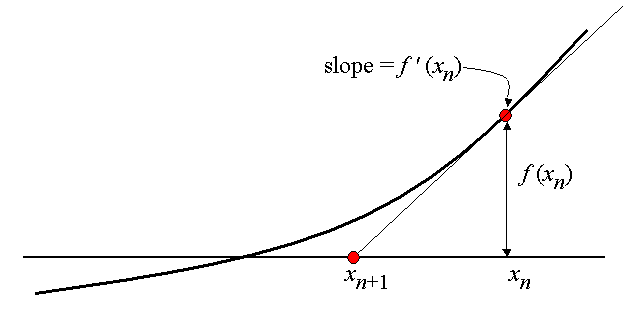
\includegraphics[scale=0.3]{img/NewtonRaphson}
\caption{Newton-Raphsone example.}
\end{figure}

\begin{equation}
\begin{aligned}
f'(x_n) = -\frac{f(x_n)-0}{x_n -x_{n+1}}\\
\Rightarrow x_{n+1} = x_n -\frac{f(x_n)}{f'(x_n)}
\end{aligned}
\end{equation}
Instead of finding the point for which $f(x)=0$, we want to find the point where its derivative is $0$. Hence we substitute $f(x)$ with $f'(x)$ and $f'(x)$ with $f''(x)$. In this way the method can be used to find points where the gradient passes through $0$, i.e., minima, maxima and points of inflections:
\begin{equation}
\begin{aligned}
f''(x_n) = -\frac{f'(x_n)-0}{x_n -x_{n+1}}\\
\Rightarrow x_{n+1} = x_n -\frac{f'(x_n)}{f''(x_n)}
\end{aligned}
\end{equation}
When dealing with vectors, $f'(x)$ is replaced by the vector of partial derivatives evaluated at $x_n$ and $\frac{1}{f''(x_n)}$ is replaced by the inverse of the Hessian matrix $\frac{-\partial^2 f(x)}{\partial \x \partial \x^T}$.

\paragraph{Derivation}
As already done, instead of maximizing the function itself, we maximize its logarithmic. Apart from the mathematical convenience this is also the advantage of avoiding underflow: we are dealing with probabilities, numbers between $0$ and $1$ and these might be too small to have a sufficient numerical precision. As the numbers go to $0$,the logarithmic makes the number goes to infinity, guaranteeing a better numerical precision.
 Since we cannot compute the derivative and set it to $0$, we use the Newton-Raphson procedure. Let us call the numerator $g(\be,\X,\y) = Pr(\y|\be,\X)Pr(\be|\X)$:

\begin{equation}
\be' = \be - \br{\frac{\partial^2\log g(\be,\X,\y)}{\partial \be \partial \be^T}}^{-1} \frac{\partial \log g(\be,\X,\y)}{\partial \be}
\end{equation}

The procedure is iterative and stops when the gradient is $0$. To check the point we have converged to corresponds to a minimum we check the Hessian matrix is negative definite.

Before computing the derivatives we re-express $g(\be,\X,\y)$.

\begin{equation}
\begin{aligned}
&\log g(\be,\X,\y) = \sum_{n=1}^N \log Pr(Y_n=y_n|\x_n, \be) + \log Pr(\be|\sigma^2) = \\
&=  \sum_{n=1}^N \log \left[\br{\frac{1}{1+e^{-\be^T\x_n}}}^{y_n} \br{\frac{e^{-\be^T\x_n}}{1+e^{-\be^T\x_n}}}^{1-y_n}\right] + \log Pr(\be|\sigma^2) =
\end{aligned}
\end{equation}
We denote $P_n=P(Y_n=1|\be, \x_n) = \frac{1}{1+e^{-\be^T\x_n}}$:
\begin{equation}
\begin{aligned}
&\log g(\be,\X,\y) =  \sum_{n=1}^N \log P_n^{y_n} +\log(1-P_n)^{1-y_n}+ \log Pr(\be|\sigma^2) =
\end{aligned}
\end{equation}
Recalling
\begin{equation}
\begin{aligned}
Pr(\be|\sigma^2)  =& \frac{1}{\sqrt{(2\pi)^D|\Sigma|}} e^{-\frac{\br{\be-\cancel{\mu}}^T\br{\be-\cancel{\mu}}}{2\sigma2}}\\
\Rightarrow\log g(\be,\X,\y) =&  \sum_{n=1}^N \log P_n^{y_n} +\log(1-P_n)^{1-y_n} -\frac{D}{2}\log(2\pi) - D\log\sigma +\\
&- \frac{1}{2\sigma^2} \be^T\be
\end{aligned}
\end{equation}

Now we can take the derivative:
\begin{equation}
\label{devg}
\begin{aligned}
&\frac{\partial \log g(\be,\X,\y)}{\partial \be} = - \frac{1}{\sigma^2} \be + \sum_{n=1}^N \frac{y_n}{P_n}\frac{\partial P_n}{\partial \be} + \frac{1-y_n}{1-P_n}\frac{\partial (1-P_n)}{\partial \be} =\\
&=\frac{\partial \log g(\be,\X,\y)}{\partial \be} = - \frac{1}{\sigma^2} \be + \sum_{n=1}^N \frac{y_n}{P_n}\frac{\partial P_n}{\partial \be} - \frac{1-y_n}{1-P_n}\frac{\partial P_n}{\partial \be}
\end{aligned}
\end{equation}

Now we must calculate $\frac{\partial P_n}{\partial \be}$:
\begin{equation}
\label{devPn}
\begin{aligned}
\frac{\partial P_n}{\partial \be} =& \frac{\partial}{\partial \be} \frac{1}{1+e^{-\be^T\x_n}} = \frac{\partial}{\partial \be} \br{1+e^{-\be^T\x_n}}^{-1} =\\
=& \frac{1}{\br{1+e^{-\be^T\x_n}}^2}  \frac{\partial}{\partial \be} \br{1+e^{-\be^T\x_n}} = \\
=&  -\x_n \frac{e^{-\be^T\x_n}}{\br{1+e^{-\be^T\x_n}}^2}   = -x_n \frac{1}{\br{1+e^{-\be^T\x_n}}}\frac{e^{-\be^T\x_n}}{\br{1+e^{-\be^T\x_n}}} =\\
=& -\x_nP_n \br{1-P_n}
\end{aligned}
\end{equation}
Substituting in \autoref{devg}:
\begin{equation}
\begin{aligned}
\frac{\partial \log g(\be,\X,\y)}{\partial \be} =&  - \frac{1}{\sigma^2} \be + \sum_{n=1}^N \frac{y_n}{P_n}\frac{\partial P_n}{\partial \be} - \frac{1-y_n}{1-P_n}\frac{\partial P_n}{\partial \be} =\\
=&- \frac{1}{\sigma^2} \be + \sum_{n=1}^N \frac{y_n}{P_n}\left[-\x_nP_n \br{1-P_n}\right]+ \\
&\quad  - \frac{1-y_n}{1-P_n}\left[-\x_nP_n \br{1-P_n}\right] =\\
=& - \frac{1}{\sigma^2} \be + \sum_{n=1}^N -y_n\x_n \br{1-P_n} - (1-y_n)(-\x_nP_n ) = \\
=& - \frac{1}{\sigma^2} \be + \sum_{n=1}^N \x_n (y_n-P_n)
\end{aligned}
\end{equation}

Now we must compute the Hessian matrix:
\begin{equation}
\begin{aligned}
&\frac{\partial^2 \log g(\be,\X,\y)}{\partial \be \partial\be^T}  = \frac{\partial}{\partial \be^T} \br{- \frac{1}{\sigma^2} \be + \sum_{n=1}^N \x_n (y_n-P_n)} =
\\ &=- \frac{1}{\sigma^2} \I -\sum_{n=1}^N \x_n \frac{\partial P_n}{\partial \be^T} = - \frac{1}{\sigma^2} \I - \sum_{n=1}^N \x_n \x_n^TP_n \br{1-P_n}
\end{aligned}
\end{equation}
where we used the result from \autoref{devPn}.

Note that the 2 terms are negative definite, hence the Hessian is always negative definite. Therefore there can only be one optimum and it must be the minimum.

The decision boundary is the one for which $Pr(Y_n=1|\x,\hat{\be}=0.5)$.

The steps above can be done for any prior and likelihood combination. In some cases the posterior might have several maxima and or some minima and it become difficult to know if the maximum is a global optimum.


The \textit{Elements of Statistical Learning} book instead of maximizing posterior (or equivalently the numerator), it maximizes the likelihood.
Let us express $Pr\left(G=k|X=x\right)=p_k(x,\theta)$ with $\theta = \left\lbrace \beta_{10},\beta_1^T,\cdots, \beta_{\left(K-1\right)0},\beta_{K-1}^T\right\rbrace$
and let us define the log-likelihood
\begin{equation}
\ell(\theta) = \sum_{i=1}^N \log p_{g_i}\left(x_i, \theta\right)
\end{equation}

Consider just two classes with responses $0$, $1$ and let $p_1(x,\theta) =p(x,\theta) $ and $p_2(x,\theta) =1-p(x,\theta)$. Recall that having two classes $\sum_{\ell=1}^{K-1} e^{\beta_{l0}+\beta_\ell^Tx_i} = e^{\beta_{10}+\beta_1^Tx_i}$. The log-likelihood can be written as:
\begin{equation}
\begin{aligned}
&\ell(\beta) = \sum_{i=1}^N \left\lbrace y_i \log p\left(x_i,\beta\right) + \left(1-y_i\right) \log \left(1-p\left(x_i,\beta\right)\right)\right\rbrace =\\
&=\sum_{i=1}^N y_i \log \frac{e^{\beta_{10} +\beta_{1}^T x_i}}{1+\sum_{\ell=1}^{K-1} e^{\beta_{l0}+\beta_\ell^Tx_i}}  +\\
& \quad\quad + \sum_{i=1}^N \left(1-y_i\right) \log \left(1-\frac{e^{\beta_{10} +\beta_{1}^T x_i}}{1+\sum_{\ell=1}^{K-1} e^{\beta_{l0}+\beta_\ell^Tx_i}}\right)= \\
&= \sum_{i=1}^N  y_i \log \frac{e^{\beta_{10} +\beta_{1}^T x_i}}{1+e^{\beta_{10}+\beta_1^Tx_i}} + \\
&\quad\quad +\sum_{i=1}^N  \left(1-y_i\right) \log \left(1-\frac{e^{\beta_{10} +\beta_{1}^T x_i}}{1+e^{\beta_{10}+\beta_1^Tx_i}}\right) = \\
&=\sum_{i=1}^N y_i \left(\log e^{\beta_{10} +\beta_{1}^T x_i} -\log \left(1+ e^{\beta_{10}+\beta_1^Tx_i}\right) \right) + \\
& \quad\quad + \sum_{i=1}^N  \left(1-y_i\right) \log \frac{1}{1+ e^{\beta_{10}+\beta_1^Tx_i}} = \\
&=\sum_{i=1}^N y_i \left(\log e^{\beta_{10} +\beta_{1}^T x_i} -\log \left(1+ e^{\beta_{10}+\beta_1^Tx_i}\right) \right) + \\
& \quad\quad - \sum_{i=1}^N\left(1-y_i\right) \log \left(1+ e^{\beta_{10}+\beta_1^Tx_i}\right) = \\
&=\sum_{i=1}^N \left\lbrace y_i \left(\beta_{10} +\beta_{1}^T x_i \right) -log \left(1+ e^{\beta_{10}+\beta_1^Tx_i}\right) \right\rbrace
\end{aligned}
\end{equation}
Here $\beta = \left[ \beta_{10}, \beta_1\right]$. To maximize the log-likelihood we set the derivative to $0$:
\begin{equation}
\frac{\partial \ell(\beta)}{\partial \beta} = \sum_{i=1}^N x_i  (y_i - p(x_i, \beta) = 0
\end{equation}

Using the \textit{Newton-Raphson} algorithm that requires the second-derivative:
\begin{align}
&\frac{\partial^2 \ell(\beta)}{\partial \beta \partial \beta^T} = -\sum_{i=1}^N x_ix_i^T   p(x_i, \beta) (1-p(x_i, \beta)\\
&\Rightarrow \beta^{new} = \beta^{old} - \left( \frac{\partial^2 \ell\left( \beta\right) }{\partial \beta \partial \beta^T} \right)^{-1}\frac{\partial \ell(\beta)}{\partial \beta}
\end{align}
Using the matrix notation,
\begin{align}
\frac{\partial \ell(\beta)}{\partial \beta} =  X^T (y-p) \\
\frac{\partial^2 \ell(\beta)}{\partial \beta \partial \beta^T} = -X^TWX
\end{align}
So the Newton step becomes

\begin{equation}
\begin{aligned}
&\beta^{new} = \beta^{old} +(X^TWX)^{-1}X^T(y-p) = \\
&=(X^TWX)^{-1}X^TW\left(X\beta^{old}+W^{-1} \left(y-p\right)\right) =\\
&= \left(X^TWX\right)^{-1} X^TWz
\end{aligned}
\end{equation}
with
\begin{equation}
z = X\beta^{old}+ W^{-1} (y-p)
\end{equation}
sometimes known as the adjusted response. This algorithm is known as \textbf{iteratively reweighted least squares (IRLS)} since each iteration solves the weighted least square problem:
\begin{equation}
\beta^{new} \leftarrow \argmin{\beta}{\left(z-X\beta\right)^TW\left(z-X\beta\right)}
\end{equation}
$\beta=0$ seems a good starting value. Convergence is never guaranteed but typically the algorithm does converge, since the log-likelihood is concave but overshooting can occur. In the rare cases that the log-likelihood decreases, step size halving will guarantee convergence.

For $K>2$ we still use the iteration procedure but we will have a $K-1$ vector response and a non-diagonal weight matrix per observation. In this case it is better to work with the vector $\theta$ directly.

\subsubsection{Second method: Laplace approximation}
There are many approximation methods but the most common is the Laplace approximation. The idea is to approximate the density of interest with a Gaussian.

Choosing a Gaussian means choosing a proper variance and mean value. The Laplace approximation method fixes one of the two parameters, i.e., the mean to the value maximizing the posterior, $\beta$. We approximate $\log g(\be,\X,\y)$ with the Taylor expansion around $\hat{\be}$:
\begin{equation}
\label{Taylor}
\begin{aligned}
\log g(\be,\X,\y) \approx &\log g(\hbe,\X,\y) + \cancel{\frac{ \partial \log g(\be,\X,\y)}{\partial \be}\bigg\rvert_{\hbe}\br{\be -\hbe}} + \\
&+ \frac{ \partial^2 \log g(\be,\X,\y)}{\partial \be^2}\bigg\rvert_{\hbe}\br{\be -\hbe}^2 =\\
&=\log g(\hbe,\X,\y)+ \frac{ \partial^2 \log g(\be,\X,\y)}{\partial \be^2}\bigg\rvert_{\hbe}\frac{\br{\be -\hbe}^2}{2}
\end{aligned}
\end{equation}

where the second term is the gradient evaluated at the maximum point that therefore must be $0$.

The Gaussian density and its log are the following:
\begin{equation}
\begin{aligned}
&\frac{1}{2\pi}e^{-\frac{(\be-\hbe)^2}{2\sigma^2}}\\
\Rightarrow &\log const -\frac{1}{2\sigma^2}\br{\be-\mu}^2
\end{aligned}
\end{equation}
which is similar to \autoref{Taylor}. By analogy of the two equations:
\begin{equation}
\begin{aligned}
&\mathbf{\mu} = \hbe\\
&-\frac{1}{\sigma^2} = -\frac{ \partial^2 \log g(\be,\X,\y)}{\partial \be^2}\bigg\rvert_{\hbe}
\end{aligned}
\end{equation}

It can be applied also to multivariate densities  $Pr(\be,\X,\y) \approx \CMcal{N}(\mathbf{\mu, \Sigma})$:
\begin{equation}
\begin{aligned}
&\mathbf{\mu} = \hbe\\
&\Sigma^{-1} = -\frac{ \partial^2 \log g(\be,\X,\y)}{\partial \be\partial\be^T}\bigg\rvert_{\hbe}
\end{aligned}
\end{equation}

Consider a multinomial 2D Gaussian function (dimensionaity of $\be$ is 2) as in \autoref{gaussianfig} and suppose to project on the plane the points of the curve having the same value (the ellipses in the figure). The ellipses will be the combination of coefficients giving the same function value.
\begin{figure}
\centering
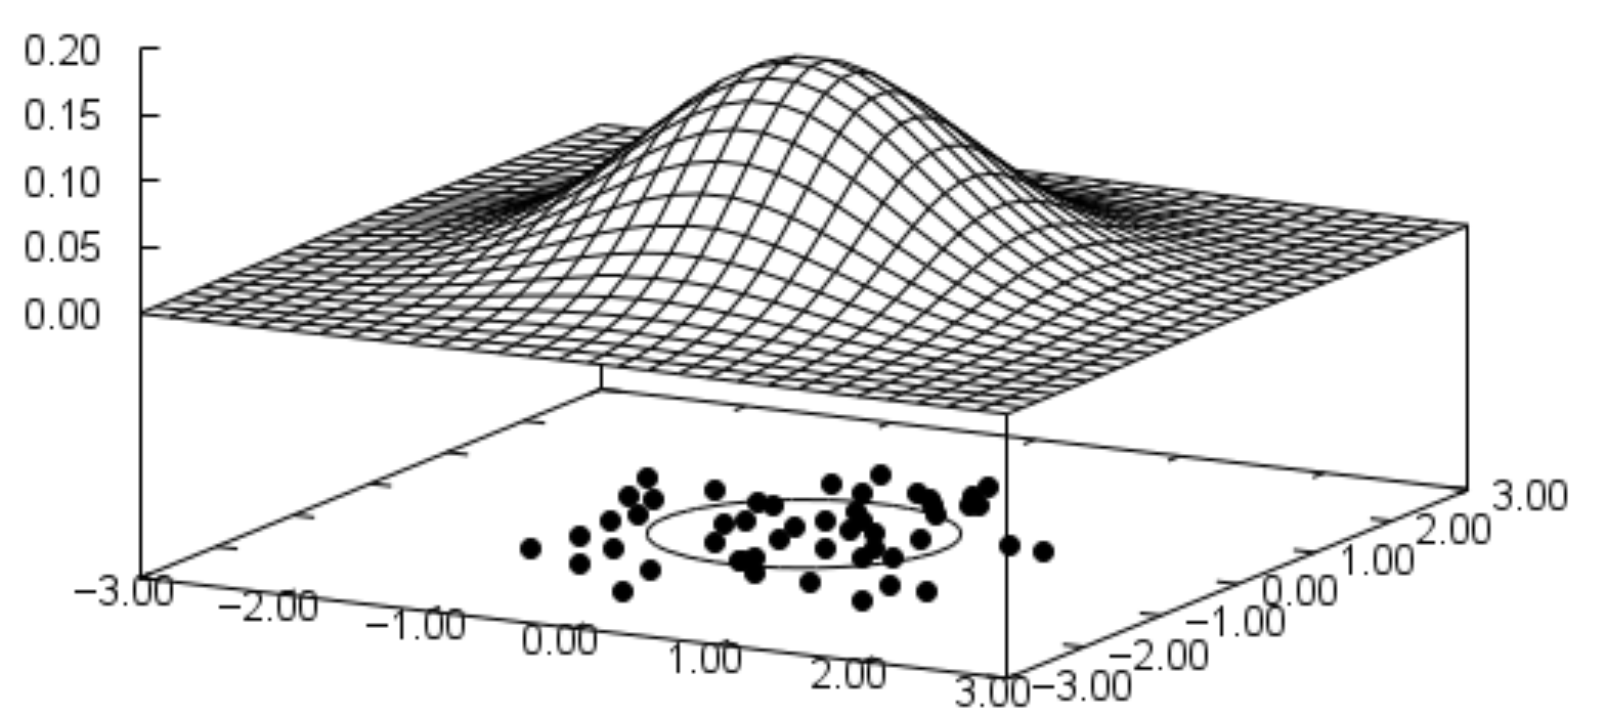
\includegraphics[scale=0.4]{img/gaussian}
\caption{Example of multinomial Gaussian.}
\label{gaussianfig}
\end{figure}

In figure \autoref{posteriorApprox} the Laplace approximation of the posterior (darker lines) is shown while the lighter lines are the true unnormalised posterior. The centre point corresponds to the maximum point $\hbe$. Note how the approximation is good around $\hbe$ and it diverges going further from it.
\begin{figure}
\centering
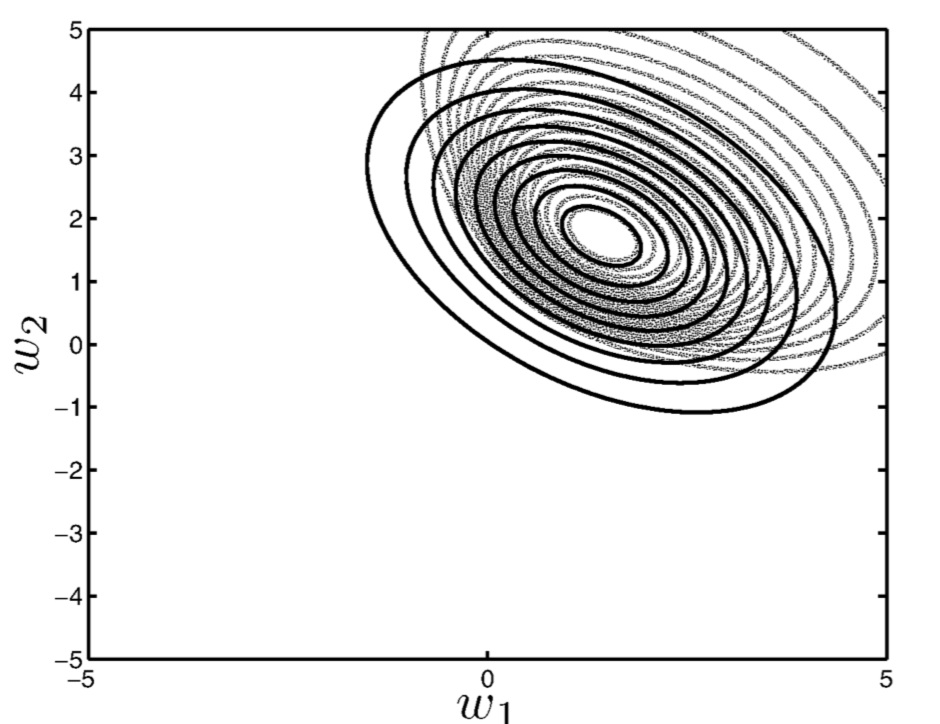
\includegraphics[scale=0.4]{img/posteriorApprox}
\caption{The axis are the parameters. The Laplace approximation of the posterior (darker lines) is shown while the lighter lines are the true unnormalised posterior. The centre point corresponds to the maximum point $\hbe$.}
\label{posteriorApprox}
\end{figure}

We use the approximate posterior to compute predictions. But now we have a density and not a single value: the prediction is computed by averaging over this density: it is like averaging over all possible values of $\be$. We should calculate the expected value $Pr(Y_{new} = 1|\x_{new}, \be)$ with respect to the approximate posterior denoted as $\CMcal{N}(\mathbf{\mu, \Sigma})$:
\begin{equation}
Pr(Y_{new}=1|\x_{new}, \X, \be) = \E_{\CMcal{N}(\mathbf{\mu, \Sigma})}\left\lbrace Pr(T_{new}=1| \x_{new}, \be)\right\rbrace
\end{equation}
However, we cannot compute the integral (of the expectation), but we can sample from $\CMcal{N}(\mathbf{\mu, \Sigma})$ and approximate the expectation with a sum:
\begin{equation}
\label{approxDen}
Pr(Y_{new}=1|\x_{new}, \X, \be) = \frac{1}{N_s}\sum_{s=1}^{N_s}\frac{1}{1+e^{-\be_s^T \x_{new}}}
\end{equation}

\paragraph{\textbf{Comparison between the decision boundaries of MAP and Laplace method.}} In case of MAP estimation we get a single separating line as in \autoref{MAP1} for the example of two classes. In case of Laplace approximation we don't have a single separating line but a density distribution. \autoref{laplace1} shows 20 boundaries (i.e., set of coefficients) sampled randomly from the distribution. All or almost all separates the classes quite well but in the area from the graph further from the classes (or from the centroids or clusters) there is a lot of variability. This variability represents the uncertainty of the classifier in those area far from the classes, where no event (in the sense of data entry) was observed.

This is made clearer by looking at the decision boundaries in \autoref{MAP2} and \autoref{laplace2}. In case of MAP it is quite obvious: the probability increases or decreases just moving close to or far from to the boundary. In case of Laplace approximation the contours are no longer straight lines. The probability are now close to $0.5$ in all the area except those closes to the two classes. It is like the classifier is unable to take a decision in those areas, that are the ones where no event has been noted.

On the contrary the classifier resulting from MAP approximation is always sure about its work: it can only classify either with one or the other class except in on the points on the boundaries. This result from the fact that it is the result of a single point and not a distribution: i.e., the amount of confidence on the result is left out.

\begin{figure}
\begin{subfigure}[t]{0.5\textwidth}
\centering
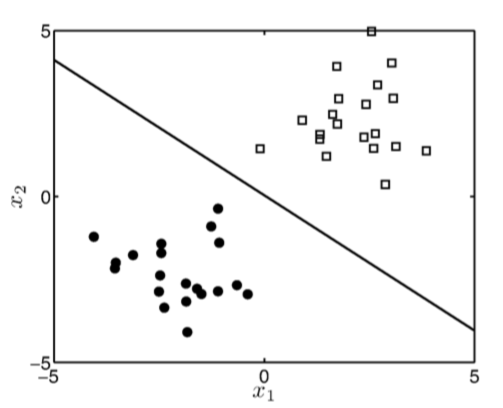
\includegraphics[width=0.85\linewidth]{img/MAP1}
\caption{Decision boundary for MAP estimation.}
\label{MAP1}
\end{subfigure}
\hfill
\begin{subfigure}[t]{0.505\textwidth}
\centering
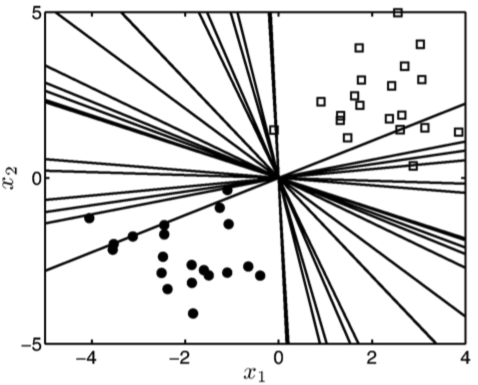
\includegraphics[width=0.8\linewidth]{img/laplace1}
\caption{Decision boundary for Laplace approximation estimation.}
\label{laplace1}
\end{subfigure}
\begin{subfigure}[t]{0.5\textwidth}
\centering
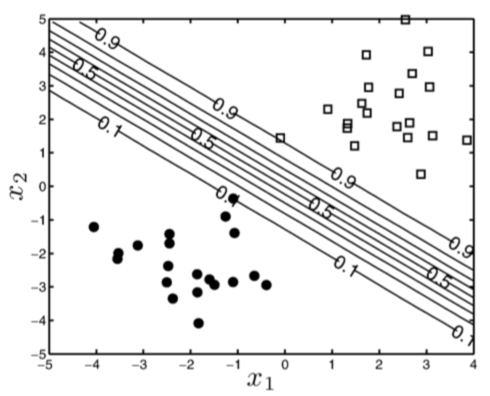
\includegraphics[width=0.8\linewidth]{img/MAP2}
\caption{Contours of probability of belonging to class 1 in case of MAP estimation.}
\label{MAP2}
\end{subfigure}
\hfill
\begin{subfigure}[t]{0.5\textwidth}
\centering
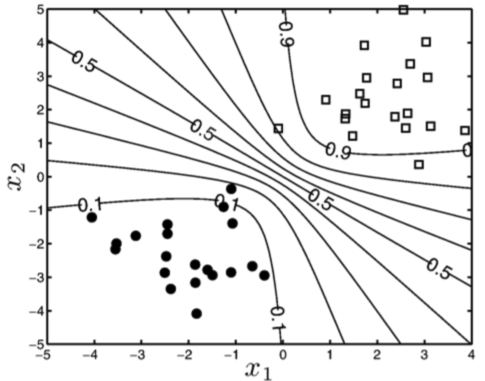
\includegraphics[width=0.8\linewidth]{img/laplace2}
\caption{Contours of probability of belonging to class 1 in case of Laplace approximation estimation computed with a sample based approximation.}
\label{laplace2}
\end{subfigure}
\caption{Comparison between MAP and Laplace approximation contours and probability densities.}
\end{figure}

\subsubsection{Third method: sampling technique	}
The reason of estimating the posterior density with Laplace approximation or any other method is to take into account uncertainties in $\be$ when making predictions. Using the Gaussian approximation we were able to sample as in equation \autoref{approxDen} directly from data. When deciding we take the conditional probability by averaging all over the potential values $\be$ by taking the expectation:
\begin{equation}
Pr(T_{new}=1| x_{new}, \X, \y, \sigma^2) = \E_{Pr(\be|\X, \y, \sigma^2)}\br{Pr(T_{new}=1|x_{new},\be}
\end{equation}

In these types of approximations we cut off the approximation step and sample directly from the posterior. A set of samples from the true posterior could be substituted directly into equation \autoref{approxDen} to compute the desired predictive probability $Pr(y_i|\x_i, \X, \be)$. A popular sampling technique is the \textbf{Metropolis-Hastings} algorithm.

Drawing from the posterior does not mean we can write it down but that we sample directly the system (physical or whatever) generating the data.

\paragraph{The metropolis-Hastings algorithms}
The objective is to sample from $Pr(\be|\X,\y,\sigma^2)$ to approximate the following expectation:
\begin{equation}
\begin{aligned}
Pr(Y_{new}&=1|x_{new},\X,\y,\sigma^2) = \E_{Pr(\be|\X,\y,\sigma^2)}\left[Pr(T_{new}=1|x_{new},\be) \right] \\
&=\int Pr(Y_{new}=1|x_{new},\be)Pr(\be|\X,\y,\sigma^2) d\be
\end{aligned}
\end{equation}
with 

\begin{equation}
\begin{aligned}
Pr(Y_{new}&=1|x_{new},\X,\y,\sigma^2) \approx \frac{1}{N_s}\sum_{s=1}^{N_s} Pr(Y_{new}=1|x_{new}, \be_s)
\end{aligned}
\end{equation}
The algorithm generates a sequence of samples $\be_1, \be_2, \cdots$. First all the algorithm is independent from the starting point, as long as we sample long enough: it is guaranteed the sequence converges.
\paragraph{\textbf{The generation of new samples}} happens in this way. Suppose we have the sample $s-1$, we will propose a new sample $\tilde{\be_s}$ and define the density $Pr(\tilde{\be}_s|\be_{s-1})$. This density is unrelated with the posterior $Pr(\be|\X,\y,\sigma^2)$ and we can define it as we please but it will affect the convergence time. A common choice is to use a Gaussian centred on the current sample, $\be_{s-1}$:
\begin{equation}
Pr(\tilde{\be}_s|\be_{s-1}, \Sigma) =\CMcal{N}(\be_{s-1}, \Sigma)
\end{equation}
Generally $\sigma$ is taken diagonal with same values. The smaller the elements on the diagonal, the smaller the distance at each step.

Such a sequence creates a \textbf{random walk}. The choice of the Gaussian is justified bye the easy of sampling from the Gaussian and by its symmetry: moving from $\tilde{\be}_{s-1}$ to $\tilde{\be}_s$ is just as likely to move from $\tilde{\be}_s$ to $\tilde{\be}_{s-1}$:
\begin{equation}
Pr(\tilde{\be}_s|\be_{s-1}, \Sigma)  = Pr(\tilde{\be}_{s-1}|\be_{s}, \Sigma) 
\end{equation}
\textbf{Accepting or rejecting the candidate $\tilde{\be}_s$} is performed by calculating the following quantity:
\begin{equation}
r = \frac{Pr(\tilde{\be}_s|\X, \y, \ssq)}{Pr(\be_{s-1}|\X, \y, \ssq)}\frac{Pr(\be_{s-1}|\tilde{\be}_s, \Sigma)}{Pr(\hat{\be}_{s}|\be_{s-1}, \Sigma)}
\end{equation}
The expression is the product of the ratio of the posterior density at the proposed sample to that at the old sample times the ratio of the proposed densities. For the Gaussian symmetry discussed above, this term is $1$ when using Gaussian densities. Note that we cannot compute exactly the densities, but being a ratio the normalisation constant (the denominator in Bayes expression) simplifies and only the likelihoods times the priors are left:
\begin{equation}
r = \frac{Pr(\tilde{\be}_s|\ssq)}{Pr(\be_{s-1}| \ssq)} \frac{Pr(\y|\X, \tilde{\be}_s, \ssq)}{Pr(\y|\X, \be_{s-1}, \ssq)}
\end{equation}
If $r>1$, i.e, we get a higher posterior density, we accept the candidate otherwise we accept the candidate with probability equal to $r$. The complete algorithm is depicted in \autoref{MHAlgo} where a uniform distribution in $[0,1]$ is used as decision rule in case $r<1$. Being a uniform distribution, the probability that $u \le r$ is $r$.

\begin{figure}
\centering
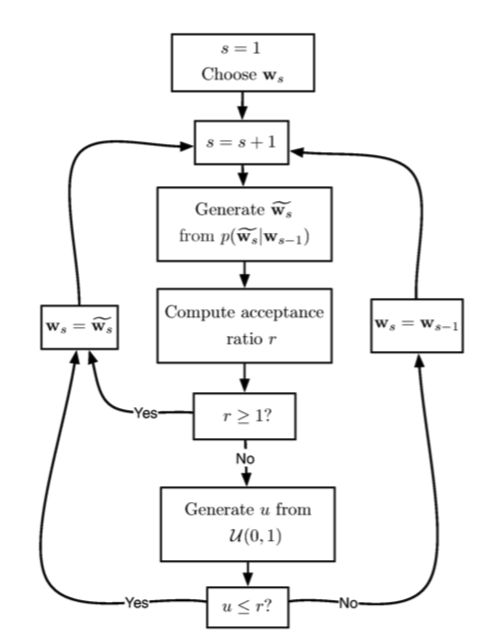
\includegraphics[scale=0.45]{img/MHAlgo}
\caption{The steps of the Metropolis-Hastings algorithm. $U$ is a uniform distribution in $[0,1]$}
\label{MHAlgo}
\end{figure}

\autoref{randomWalk} shows a 10-iteration process of the algorithms where solid lines are accepted coefficients, dashed lines are the rejected ones. Note that even the third sample causes a decrease in the posterior $r<1$, nevertheless in this specific case the decision rule accepted it. On the contrary the 4-th sample causes a huge decrease hence it is very unlikely it is accepted and in fact it is not, so $\be_4 = \be_3$. After $N$ samples we compute the sample based approximations to the mean and covariance
\begin{equation}
\begin{aligned}
\mu' &= \frac{1}{N_s} \sum_{s=1}^{N_s} \be_s\\
S' &= \frac{1}{N_s} \sum_{s=1}^{N_s} (\be_s-\mu')(\be_s-\mu')^T
\end{aligned}
\end{equation}

\begin{figure}
\centering
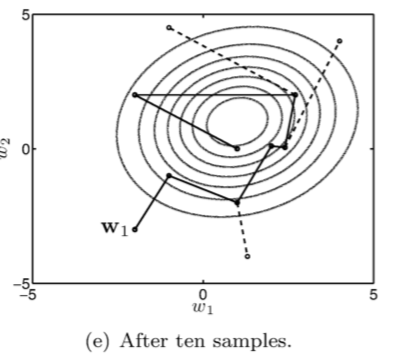
\includegraphics[scale=0.4]{img/randomWalk}
\caption{Example of Metropolis-Hastings iterations: solid lines are accepted coefficients, dashed lines are the rejected ones.}
\label{randomWalk}
\end{figure}

\begin{definition}{\textbf{Burn-in}} It is the time interval between the starting of the algorithm and the convergence. 
\end{definition}
It cannot be determined: to overcome this problem, a method for determining convergence (to a distribution, not to a value) should be established. For example, in the algorithm above, we do not know if the starting point belongs to an area from which we are supposed to sample: it might be very far from the posterior. Including these samples in the approximation might result in a not good value. That is why the first samples (ranging from few samples to thousands) should be discarded.

A popular method is to start several samplers simultaneously from different starting points. When all the samplers are generating samples with similar mean and variance, it suggests they converged all to the same distributions.

\begin{definition}{\textbf{convergence} In this case we are talking about the convergence to a given distribution, not a single point. The convergence to a distribution is characterized to the convergence of its parameters: in case of the Gaussian the mean and variance.}
\end{definition}

We can even look at each coefficient independently:
\begin{equation}
Pr(\be_1|\X,\y,\sigma^2) = \int Pr(\be_1,\be_2|\X,\y,\sigma^2) d\be_2
\end{equation}

\paragraph{\textbf{To calculate the predictive probability}} using the obtained set of samples, we can do what already done with the Laplace approximation:
\begin{equation}
Pr(Y_{new}=1|\x_{new}, \X,\y,\sigma^2) = \frac{1}{N_s} \sum_{s=1}^{N_s} \frac{1}{1+e^{-\be^T_s \x_{new}}}
\end{equation}

\begin{figure}
\begin{subfigure}{.47\textwidth}
\centering
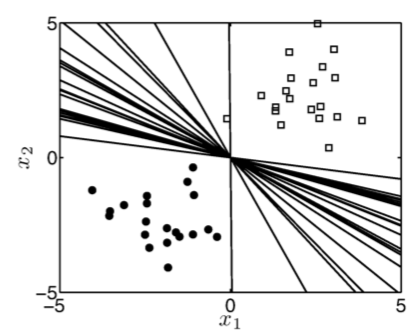
\includegraphics[width=.8\linewidth]{img/MH1}
\caption{Predictive probability contours of classifying objects as square.}
\label{MH1}
\end{subfigure}
\begin{subfigure}{.47\textwidth}
\centering
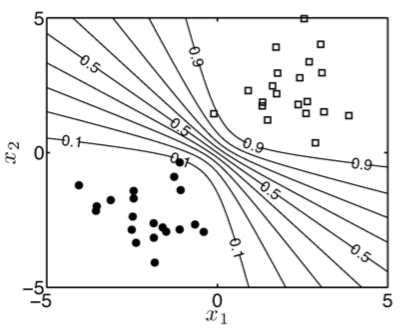
\includegraphics[width=.8\linewidth]{img/MH2}
\caption{Decision boundaries created from randomly selected MH samples.}
\label{MH2}
\end{subfigure}
\caption{Example of Metropolis-Hastings algorithm results.}
\end{figure}
\autoref{MH1} and \autoref{MH2} show an example of possible shapes of contours: it does not look too different from the Laplace ones. The only difference is that these contours are not so tight as the Laplace's ones. This suggests the probability decreases more slowly.

\paragraph{\textbf{Limitations}} The difficult mostly lies in the unknown shape of the density. When a density has two or more modes, MH moves towards the modes as these moves increase the posterior density and hence are always accepted. When close to a mode, many steps are required to move from one mode to another and this is very unlikely. We might end up exploring a mode without even knowing the other exists (see \autoref{mode1}). Another problem arises when the variables are strongly correlated (see \autoref{mode2}). Let us pick any position and propose a movement from a Gaussian with diagonal covariance (i.e., having circular contours). The shapes are very different and many samples will be rejected: the majority of moves that we sample from our proposal will involve moving steeply down the probability gradient. There are even other problems.

\begin{figure}
\begin{subfigure}{.5\textwidth}
\centering
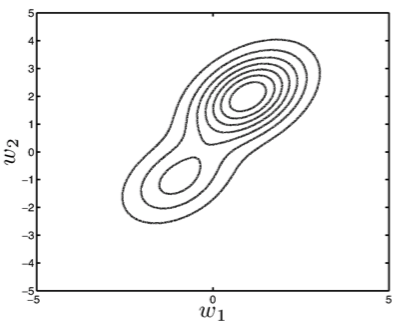
\includegraphics[width=.8\linewidth]{img/mode1}
\caption{A bi-modal density.}
\label{mode1}
\end{subfigure}
\begin{subfigure}{.5\textwidth}
\centering
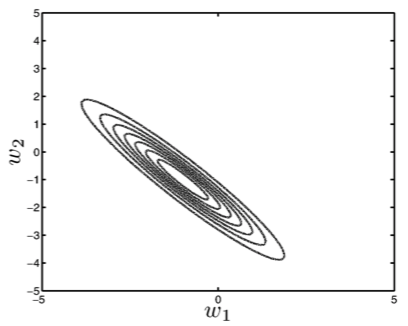
\includegraphics[width=.8\linewidth]{img/mode2}
\caption{Highly correlated parameter density.}
\label{mode2}
\end{subfigure}
\caption{Example of Metropolis-Hastings algorithm results.}
\end{figure}

\subsubsection{Usage}
LR is used as data analysis tool where the goal is to  understand the role of the input variables in explaining the outcome. Typically many models are fit in a search for a parsimonious model involving a subset of the variables, possibly with some interactions terms. 

It is widely used in biostatistical applications where binary responses (two classes) occur quite frequently. For example, patients survive or die, have heart disease or not, or a condition is present or absent.

\subsection{Regularized Logistic regression}
We can use the $L_1$ penalty for variable selection and shrinkage:

\begin{equation}
\argmax{\beta_0,\beta_1} \left\lbrace \sum_{i=1}^N y_i\left(  \beta_0 + \beta^Tx_i\right) -\log \left( 1+e^{\beta_0 + \beta^T x_i}\right) -\lambda \sum_{j=-1}^p |\beta_j|\right\rbrace
\end{equation}
This function is concave and can be solved using a nonlinear programming method.
\subsection{Logistic vs LDA}
The difference between the models relies on how the linear coefficients are estimated. The logistic regression model is more general since it makes less assumptions.

LDA is not robust to outliers since observations far from the decision boundary are used to estimate the common covariance matrix, while they are scaled down in the Logistic regression.

\subsection{Perceptron learning algorithm}
It tries to find a separate hyperplane by minimizing the distance of misclassified points to the decision boundary. If a response $y_i = 1$ is misclassified, then $x^T_i \beta + \beta_0 < 0$, and the opposite for a misclassified response with $y_i = -1$. The goal is to minimize
\begin{equation}
D(\beta, \beta_0) = - \sum_{i\in\CMcal{M}} y_i\left(x_i^T\beta + \beta_0\right)
\end{equation}
where $\CMcal{M}$ is the set of misclassified points.
The gradient is
\begin{align}
\frac{\partial D(\beta,\beta_0}{\partial \beta} = -\sum_{i\in\CMcal{M}}y_ix_i \\
\frac{\partial D(\beta,\beta_0}{\partial \beta_0} = -\sum_{i\in\CMcal{M}} y_i
\end{align}
where the algorithm uses the stochastic gradient descent where the coefficients are updated by the gradient value weighted by a step $\rho$. There are many problems though:
\begin{itemize}
\item when data are separable, there are many solutions which depend on the starting value;
\item many steps might be required;
\item when data are not separable, the algorithm will not converge;
\end{itemize}

\subsection{Optimal separating hyperplanes}
\label{OSH}
See \autoref{HardMarginSVM}.